%----------------------------------------------------------------------------------------
%	Hardware
%----------------------------------------------------------------------------------------

\chapter{Hardware Components}

\section{Final Design}
The final design contains the following functional blocks: linear voltage regulator, instrumentation amplifier, input filters, output filter, tare button, LED indicators, battery pack, and Raspberry Pico Pi. The circuit schematic is shown in Figure 
\ref{fig:altium_sche}.

\textbf{Linear Voltage Regulator}\\
The entire circuit except for the Raspberry Pico Pi is powered by 4 x AAA batteries, the voltage coming out of the battery pack typically varies over time and the voltage level drops as the batteries are being drained, therefore it needs to be regulated before supplying voltage to the rest of the circuit. This is done by connecting the battery pack to the input of the linear voltage regulator, the output of the linear voltage regulator is a 3.3V DC voltage, and is used to power the rest of the circuit.

\textbf{Wheatstone Bridge \& Instrumentation Amplifier}\\
The four strain gauges in the scale are connected in a Wheatstone bridge manner, and the voltage difference between the middle of the two legs is configured to become negative when weights are put on the scale. These two points are connected to the input terminals of the instrumentation amplifier, which amplifies the difference while also adding a positive voltage offset to the signal. This is to ensure the voltage level is suitable to be fed to the ADC unit of the Pico Pi for signal processing, the voltage offset is added in order to make full use of the voltage output range of the operational amplifier, improving accuracy.

\textbf{Input/Output Filters}\\
There is noise present in both the input signal and the output signal, first order RC filters are deployed to filter out high frequency noise, giving a more stable and accurate voltage output to be fed to the ADC.

\textbf{Tare button}\\
A push button is connected to a GPIO pin of the Raspberry Pico Pi, button press is detected by an interrupt and the tare request is handled by embedded software.

\textbf{LED indicators}\\
Four LEDs and their respective current limiting resistor are connected to GPIO pins of the Raspberry Pico Pi, on and off of these LEDs are controlled by embedded software. They are for indication purposes to communicate the status of the system to users. They indicate power, WiFi connectivity, tare button push, and successful measurement respectively.

\textbf{Battery pack}\\
Battery pack is connected to the PCB via jumper cables in the working prototype, as shown in Figure \ref{fig:battery_pack}.

\begin{figure}[h]
    \centering
    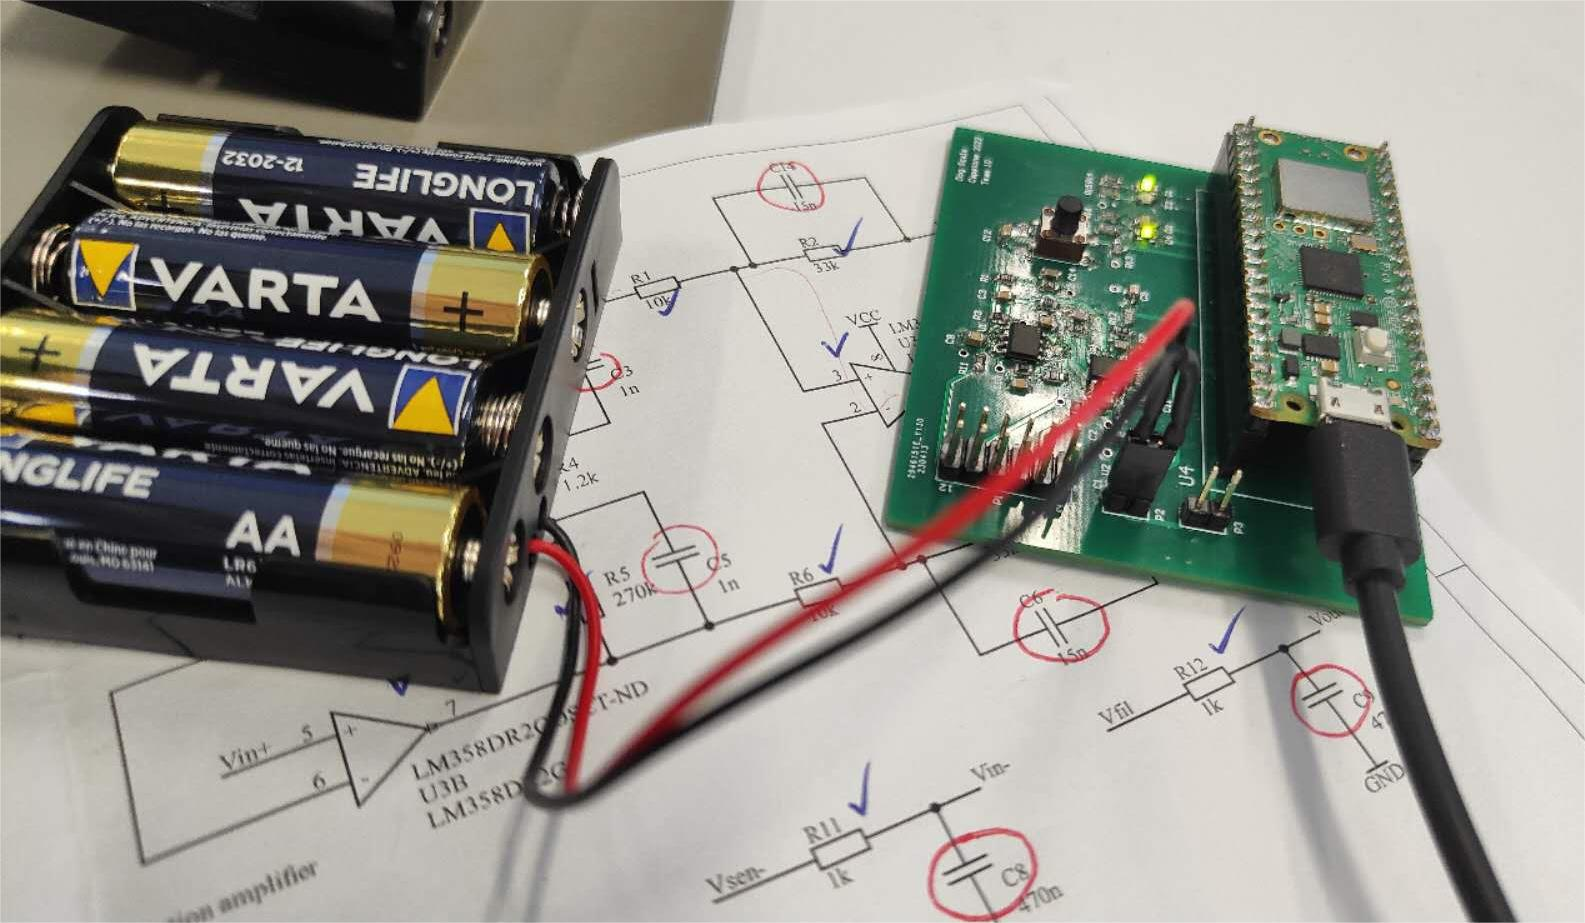
\includegraphics[width=0.5\textwidth]{final-report/assets/battery_pack.jpg}
    \caption{Battery pack connected to PCB.}
    \label{fig:battery_pack}
\end{figure}

The complete design is shown in Figure \ref{fig:altium_sche} below.

\begin{figure}[h]
    \centering
    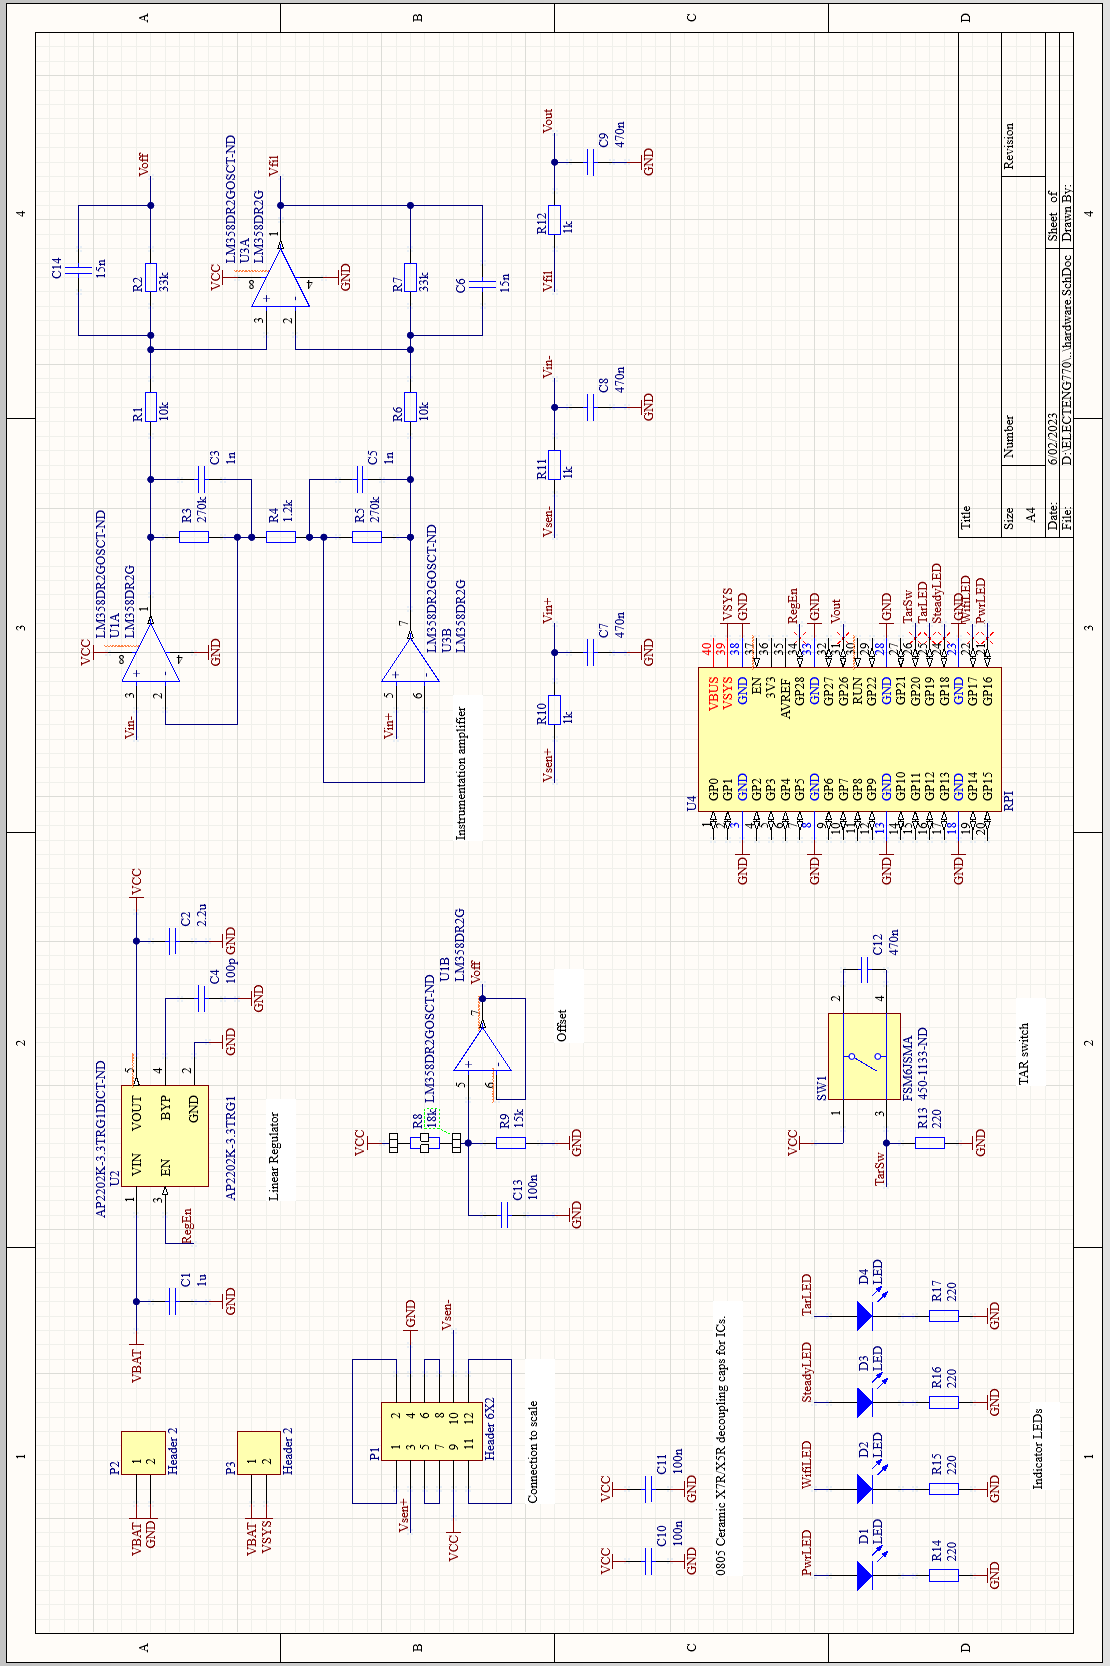
\includegraphics[width=\textwidth]{final-report/assets/altium_schematic.png}
    \caption{Altium schematic.}
    \label{fig:altium_sche}
\end{figure}

\section{Hardware Validation}
The instrumentation amplifier is simulated in LTSpice with component values shown in Figure \ref{fig:ltspice_sche}. Vcc is set to 2V instead of 3.3V to account for the output voltage swing from the positive rail as the operational amplifier we chose (LM358) is not rail-to-rail.

\begin{figure}[h]
    \centering
    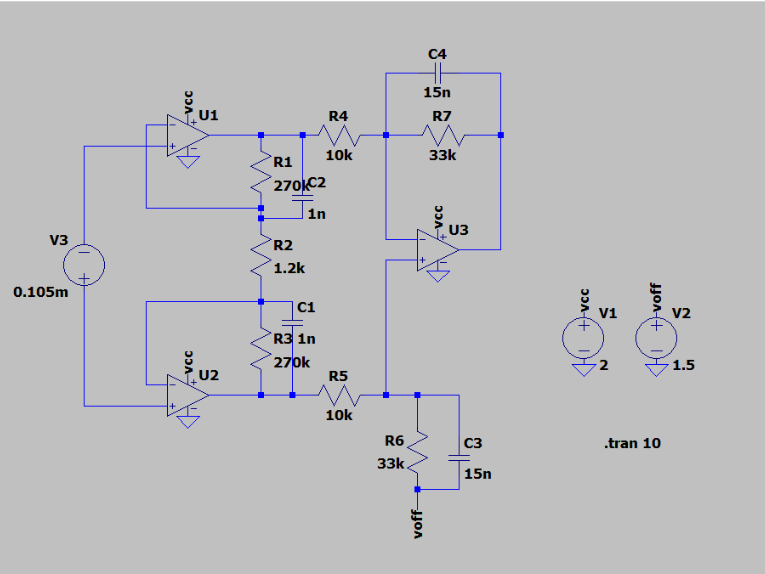
\includegraphics[width=0.45\textwidth]{final-report/assets/ltspice_sche.png}
    \caption{LTSpice schematic of the instrumentation amplifier.}
    \label{fig:ltspice_sche}
\end{figure}

Table \ref{tab:in_out_vol} summarises the input voltages and their corresponding output voltages for different weights, screenshots of the simulation result can be found in Appendix A. Experimental results closely match the simulation results, screenshots taken from the oscilloscope are found in Appendix B.

\begin{table}[h]
    \centering
    \begin{tabular}{|c|c|c|c|}
        \hline
        Weight & Input Voltage & Output Voltage (simulation) & Output Voltage (experiment) \\
        \hline
        0kg & 0.105mV & 1.656V & 1.6549V \\
        4.86kg & -0.09mV & 1.366V & 1.3748V \\
        9.76kg & -0.28mV & 1.083V & 1.0958V \\
        14.77kg & -0.47mV & 0.801V & 0.8026V \\
        20.79kg & -0.66mV & 0.518V & 0.5207V \\
        24.72kg & -0.843mV & 0.246V & 0.2459V \\
        \hline
    \end{tabular}
    \caption{Input voltage and output voltage.}
    \label{tab:in_out_vol}
\end{table}

All resistors and capacitors used in our design are 0805 SMD components with 5\% tolerances, they are manufactured by many different manufacturers and are abundant in the market. The linear voltage regulator chosen is AP2202K-3.3TRG1, of which DigiKey has a large number in stock. The operational amplifier used is LM358N, it is a common operational amplifier used in many applications and is always in stock. It is unlikely that any of the components used in our design will run out of stock in the market or become obsolete in the near future.

The largest impact the component tolerances have on our PCB is the instrumentation amplifier gain, since some resistor values mismatched and the gain was not exactly what we calculated. This could be adjusted easily by replacing some of the resistors.

The design meets all specifications outlined in Table \ref{tab:design_spec} below.

\begin{table}[h]
    \centering
    \begin{tabular}{|c|c|}
        \hline
        Parameter & Value \\
        \hline
        Supply Voltage & 4 x AA Batteries \\
        Weight Range & 0 to 25kg \\
        Weight Accuracy & 0.25kg \\
        Output Voltage Range & 0 to 3V \\
        Operating Temperature & 0 to 40°C \\
        Display & Measure success - LED Indicator \\
        Compliance & RoHS and WEEE (AS/NZS 5377) \\
        \hline
    \end{tabular}
    \caption{Design Specifications.}
    \label{tab:design_spec}
\end{table}

\section{Standard Compliance}

The linear voltage regulator, operational amplifiers, and all SMD resistors and capacitors used are chosen specifically to meet RoHS compliance, these components are free from restricted substances listed in RoHS standard, and therefore reducing the negative impact on the environment and human health. In addition, these components are designed to be easily removable from the PCB, facilitating separate collection and recycling, reducing the amount of e-waste at the end of their life cycle. We ordered these components from a local reputable distributor, reducing carbon footprint during transportation.

The regulator has an enable pin which is controlled by the embedded software, the rest of the circuit can be turned off to save power while data is being transferred to the backend, which saves power and increases service life.

We have taken the following steps to improve serviceability:
\begin{itemize}
    \item Design decisions, modifications and voltage measurements were documented throughout the design process, which enables fast troubleshooting.
    \item  Components are clearly labelled on PCB to allow for fast locating, making debugging easier.
    \item All functional blocks are modular design and therefore they can be easily replaced if one of them fails.
    \item Connectors and cables are of high quality to minimize chance of failure.
    \item Include LED indicators to communicate system status, which provides useful information for debugging.
\end{itemize}
 